\section{Logistics}
\label{sec:fdsp-tc-log}


Transporting equipment and people underground is one of the more challenging aspects of the \dword{lbnf}/\dword{dune} endeavor. Access underground goes through the mile long Ross shaft, which is now undergoing renovation. The shaft is outfitted with a single cage for people and materials and two skips that are needed to remove the rock underground. Planning for using the cage is important to making \dword{lbnf}/\dword{dune} a success. Given the enormous cost of the \dword{cf} contracts and the large cost of any inefficiencies in construction, the overall coordinator of the Ross Shaft for \dword{lbnf}/\dword{dune} will be the \dword{cf} \dword{cmgc}. Both \dword{lbnf} and \dword{dune} will also have a large number of contractors, institutions, and scientists who will need to bring equipment and materials underground. \dword{lbnf}/\dword{dune} will establish a logistics organization in South Dakota near \dword{surf} to facilitate the flow of material and people to the underground area. This organization will be responsible for receiving all goods for \dword{lbnf} (except CF) and \dword{dune},
for coordinating the transport of this material underground with the \dword{cf}-\dword{cmgc}, and
for coordinating personnel usage of the Ross cage with the \dword{cf}-\dword{cmgc}. 


%\begin{dunetable}
%[Logistics Specifications]
%{ll}
%{tab:table-Log-Req}
%{Table of logistics specifications.}
%Specifications &  \\ \toprowrule
%Material Handling & Comply with the SURF Material %Handling Specification \\ \colhline
%CMGS coordination & Provide CMGC with two-week notice %of shipments to SURF \\ \colhline
%Stage DUNE Shipments & Provide a one-month local %buffer of DUNE materials \\
%\colhline
%\dword{apa} Storage & Provide storage space for 150 %\dword{apa}s in a clean environment \\
%\colhline
%Inventory & Provide an inventory system accessible to %the collaboration \\
%\end{dunetable}
 %\fixme{Specifications table needs to be converted to official format}
 
Figure~\ref{fig:logistics-material-flow} shows a high-level overview of the material flow to the Ross shaft. Freight is delivered to a central South Dakota warehouse facility (\dword{sdwf}) except for possibly the cryogenic equipment. 
 The materials are then transported in a just-in-time to the Ross headframe where they are brought underground. For the detector, the \dword{apa} electronics and photon detector components will also be shipped to the \dword{itf} where they are assembled and then shipped back to \dword{sdwf}.
 
\begin{dunefigure}[Material flow diagram for logistics ]{fig:logistics-material-flow}
  {Material flow diagram for the LBNF/DUNE logistics.}
 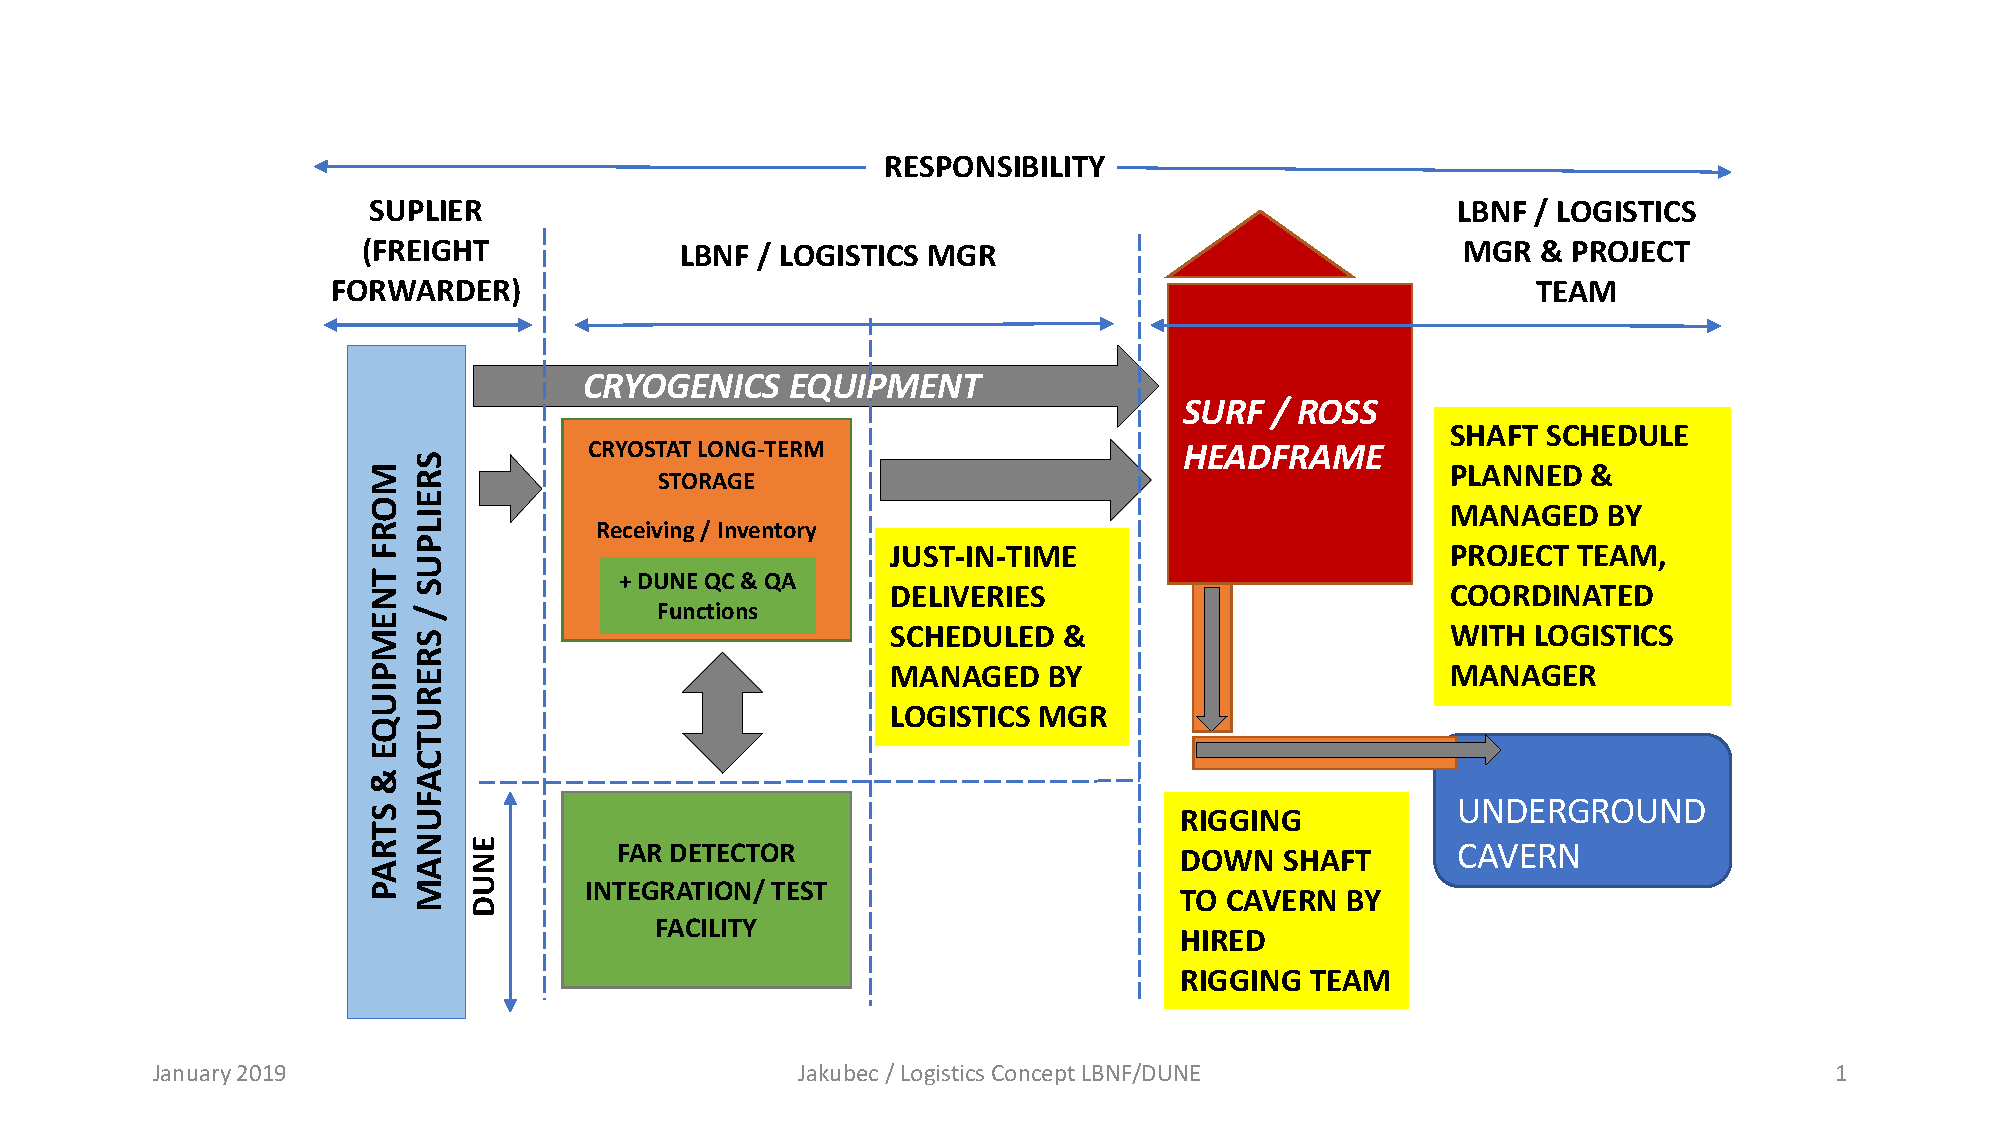
\includegraphics[width=\textwidth]{logistics-material-flow}
\end{dunefigure}


%%%%%%%%%%%%%%%%%%%%%%%%%%%%
\subsection{Logistics Planning}
\label{sec:fdsp-tc-logPln}
\dword{lbnf}/\dword{dune} logistics oversees transportation of the cryostat (steel, foam, and membrane), the cryogenic system, the detector, and all related infrastructure not provided by facilities. \dword{lbnf} specifically oversees the cryostat and cryogenics system, which will not be discussed in detail in this \dword{tdr}, but because \dword{lbnf} material dominates the logistics a summary is required. The cryostat steel structure for each cryostat requires bringing roughly 1,800 individual steel pieces underground, some which weigh up to 7.5t as well as 125t of bolts to assemble the steel pieces. The internal structure, which includes the foam insulation and the thin stainless steel membrane, will require transporting roughly 4,000 boxes, each roughly 1.5 $\times$ 3.5 $\times$ 1.2 m$^3$. The plan for cryostat installation, at present, calls for all components to be warehoused in South Dakota before installation begins. This means that the logistics operation will need roughly 5,000 m$^2$ of warehouse space approximately 2 years before beginning the installation of the first DUNE detector. By the time DUNE detector components start arriving, most of the cryostat boxes will have been removed from the warehouse, leaving ample space for the detector and cryogenics components. Additional space may be required if the boxes for the second cryostat arrive before the detector\#1 installation is complete, but several buildings of the required size are available in the area if expansion is required.


\begin{dunefigure}[Simplified model of the Ross Cage]{fig:fdsp-tc-Cage}
  {Simplified Ross Cage model.}
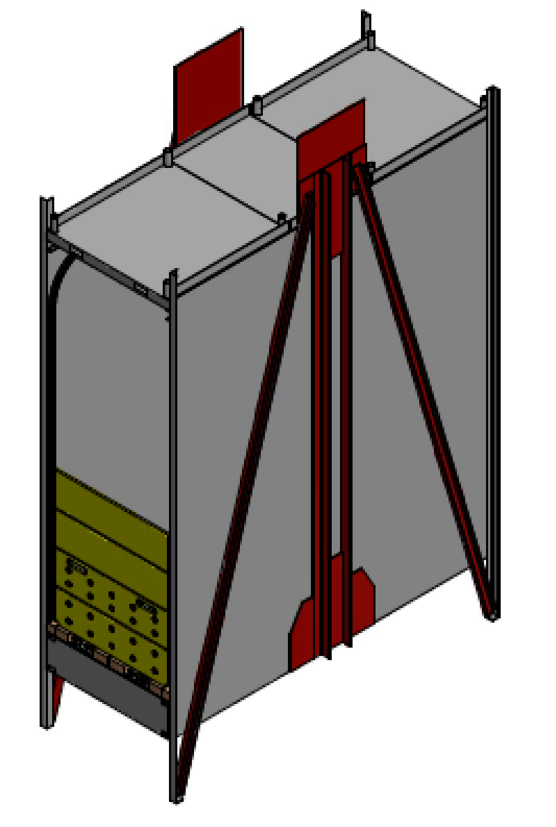
\includegraphics[width=.5\textwidth]{Cage-view}
\end{dunefigure}
%
\begin{dunetable}
[Ross Cage specifications]
{cc}
{tab:table-Ross-Cage}
{Ross Cage parameters.}
Ross Cage Parameters &  
\\ \toprowrule
Inside height &  3.6 m\\ \colhline
Inside depth & 3.7 m \\ \colhline
Inside width & 1.38 m \\
\colhline
Weight limit&  5,897 kg \\
\colhline
Round trip time & 17 min\\ \colhline
\end{dunetable}

All material brought underground must conform to the \dword{surf} Facility Access Specification \cite{bib:docdb328}. This document defines the limitations on dimensions and weights for all materials to be transported underground.  The most important limitations, which are described in detail in the specification document, relate to the Ross shaft and Ross cage. It is possible to bring material down the shaft underneath the cage as a slung load, but this is a much slower process and requires careful planning, detailed procedures, and review. The \dword{dune} \dword{apa}, for example, requires this special handling because they are too tall to fit in the cage. Most material should be brought underground inside the cage. Figure \ref{fig:fdsp-tc-Cage} shows an image of the new Ross cage and Table \ref{tab:table-Ross-Cage} summarizes its parameters. The round trip travel time for the Ross cage is 17 minutes, but the time needed to load and unload the cage as well as any slung load is more than an hour round trip because both loading/unloading and travel times are longer. 

Planning the \dword{dune} logistics is complex. The Ross headframe has no loading dock, so all materials must be transported with a flatbed or curtain-sided chassis. The equipment can then be removed with a forklift at \dword{surf}. In general, unloading at \dword{surf} must be  considered while loading trucks at the warehouse to avoid difficulties at \dword{surf} delivery. The \dword{cf}-\dword{cmgc} must coordinate all loads through the Ross shaft. To do this \dword{dune} must provide two weeks notice to incorporate an advance delivery plan into the overall hoist schedule. \dword{dune} collaborators may not ship equipment directly to the Ross Shaft unless the logistics team has coordinated the delivery. A central inventory system will capture all goods at receipt in the warehouse in South Dakota. \dword{dune} institutions must provide shipping data and consign cargo accordingly (a shipping manual will be provided by the logistics team), so the logistics team can monitor progress. 

In \dword{protodune}-\dword{sp}, delays in shipping and customs caused up to three weeks delay in the arrival of some parts, which caused significant re-planning of the installation work. To prevent this from becoming a much larger problem in \dword{dune}, a minimal one month buffer of materials will be planned. With this, the underground work can be planned well in advance, knowing all materials will be available. This will require that sufficient space be available in the warehouse and underground at \dword{surf} to house the material buffer. Many small parcels will arrive at the warehouse from different sources. The warehouse staff will de-consolidate arriving cargo as required and consolidate deliveries to \dword{itf} or \dword{surf} into larger boxes/crates, following \dword{itf} or \dword{surf} delivery plans, to make efficient use of available trucks and the Ross hoist. 


\begin{dunefigure}[Underground space needs during installation setup]{fig:fdsp-tc-setup}
  {Image showing the cavern on end opposite of the detector. During the installation setup phase, half the space will be used for the cryostat work and half for storage of the detector infrastructure. The material outside the cavern must be stored in the logistics warehouse.}
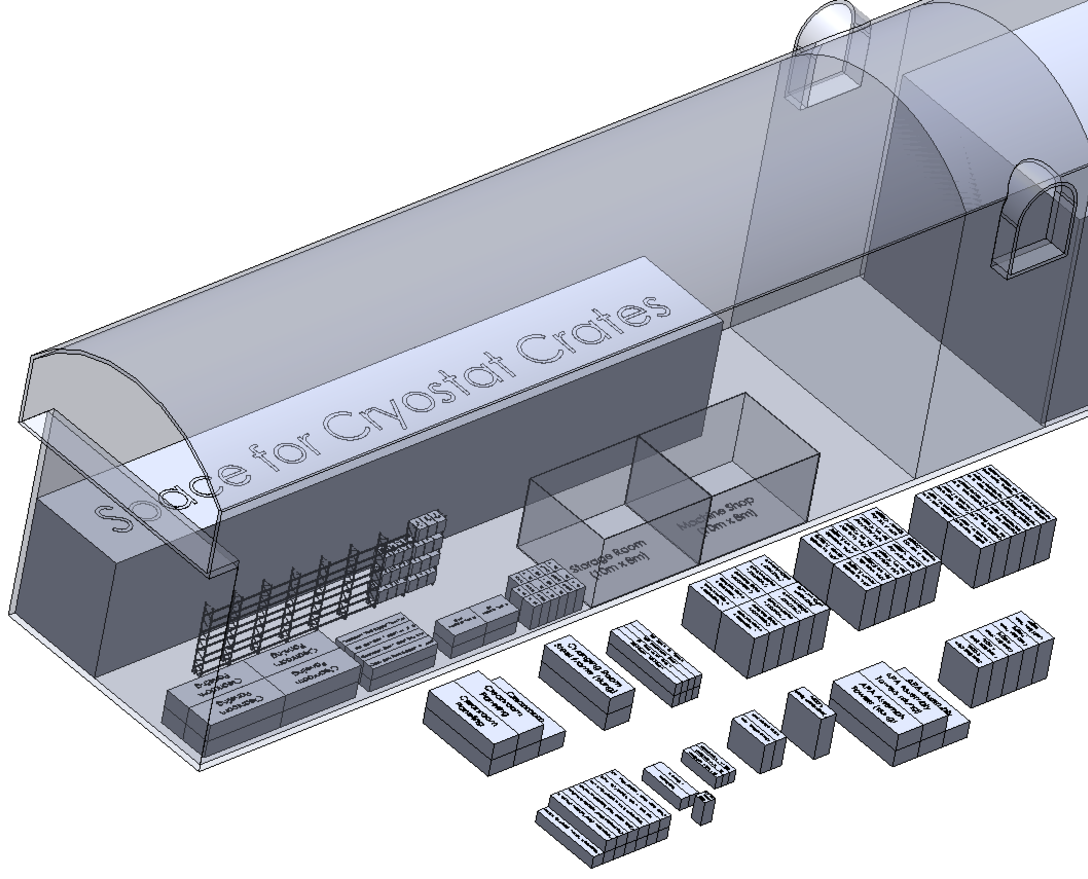
\includegraphics[width=.9\textwidth]{Material-Setup}
\end{dunefigure}
%

To discover how much space is needed for storage and how much hoist time must be dedicated to \dword{dune}, a detailed inventory of all detector equipment and \dword{dune} infrastructure is needed. The list of all the materials has been solicited from all consortia and technical coordination. The entries in the inventory spreadsheet are organized as "Loads" for the Ross shaft where a load is a crate or set of boxes that will either be transported underground in the hoist or as a slung load.\cite{bib:docdb8426}
%\href{http://docs.dunescience.org/cgi-bin/ShowDocument?docid=8426}{DUNE load Spreadsheet} \cite{bib:docdb8426}

Information captured in the load spreadsheet includes number of hoist trips, type of trip (slung load or cage), package dimensions, weight and type of package (crate, pallet, box, or carton). The load list at present predicts 1,600 hoist trips and approximately 2 months of cage time, most of which is spread over one year. The installation operation for the single-phase detector will span two years, so dividing the logistics planning into several phases is prudent. The load information is divided into the \dword{cuc} setup phase, the installation setup phase, and the detector installation phase. For each phase, a model was generated to show how much material can be stored underground outside the work area and how much material must be stored on the surface. These models set the space requirements for the logistics on the surface. The phase with the largest amount of material to transport is the detector setup phase. Figure \ref{fig:fdsp-tc-setup} shows the model of the underground area and the required boxes for surface storage for the first $1/3$\ of the setup. This represents the first month of installation setup and shows that roughly 1,000 m$^2$\ of warehouse space will be needed for \dword{dune} at this time. In addition to the space needed for receive and ship equipment underground, the warehouse will also need space to store up to 150 \dwords{apa}. This adds an additional 700 m$^2$\ to needed warehouse area. 


%%%%%%%%%%%%%%%%%%%%%%%%%%%%
\subsection{Logistics Quality Assurance and Quality Control}
\label{sec:fdsp-tc-log-qaqc}


\dword{protodune} was an extremely useful exercise in general, but we can draw only a few conclusions about \dword{dune} logistics because shipping to Europe differs from shipping to South Dakota and the CERN receiving and transport divisions will not be used for \dword{dune}. The most important lessons learned from \dword{protodune} logistics are listed below.
\begin{enumerate}
\item Lack of a central inventory system made it impossible to track shipments.
\item Delays in shipping meant that the installation work could not be planned and parts were installed as they arrived. 
\end{enumerate}

To address these issues, an inventory system will be implemented at the logistics warehouse facility, and a minimum one month material buffer will be required from the consortia in South Dakota.

We do not foresee any component testing in the warehouse, so the scope of the quality control work there is limited. A \dword{qa}/\dword{qc} component, however, will be required at receiving. One critical \dword{qc} check at the logistics facility will ensure that all materials to be shipped to the Ross headframe will fit in the cage. Moreover, if a slung load is needed, the facility will confirm that the necessary procedures are in place and approved before any material is transported to \dword{surf}. The other primary \dword{qc} function performed at the logistics facility is to inventory all shipments described below.

The contribution in kind model of this project makes logistics and inventory control as well as gathering of the relevant construction data extremely complex. Therefore, the logistics (inventory) control and collection of scientific data must be controlled by independent systems. 
The logistics supply chain will be controlled by the contributors freight forwarding system until supplies arrive at the South Dakota Warehouse Facility (\dword{sdwf}), which has yet to be defined/established.  \dword{sdwf} will be the ultimate point of capture for all \dword{lbnf}/\dword{dune} parts/equipment except possibly for the cryogenic system, given the contractual requirements.
The inventory process at the \dword{sdwf}, the \dword{itf} and the \dword{surf} receiving at Ross Shaft will be controlled by one integrated commercial warehouse management system (\dword{wms}). 

We will need some workflow functionality at \dword{itf} pre-assembly.
The \dword{wms} will provide basic receiving, inventory control, and shipping status for all parts/equipment delivered to \dword{sdwf}. That will include pre-assembled equipment, which will enter as new parts from \dword{itf} as created by the work flow.
The \dword{qc}/\dword{qa}, manufacturing, and other relevant data required by the \dword{dune} collaborators will be stored in a separate, as yet undefined and undeveloped, \dword{dune} construction database. 
This \dword{dune} construction database is independent of the \dword{wms} system, and the relevant contributing consortia are responsible for transferring the required data before shipment from supplier to the \dword{dune} construction database (\dword{dcdb}).  The \dword{wms} database will provide the relevant logistics data to the \dword{dcdb}. The form of data transfer is not yet determined.
All \dword{qc}/\dword{qa}, test, and other relevant manufacturing data will be directly input into \dword{dcdb} and will be the responsibility of the different contributing consortia. \dword{dune} must provide a \dword{qc}/\dword{qa} process for all parts/equipment received at the warehouse after being inventoried. That \dword{qc}/\dword{qa} data must be transferred directly to \dword{dcdb} by \dword{dune}. 
The \dword{dcdb} will be an integral part of the logistics, assembly, and \dword{qc}/\dword{qa} system. It must provide the \dword{itf} shipping (supply) and assembly reports and create the new equipment denomination for the \dword{wms} to register.  The \dword{dcdb} will document the \dword{itf} sub-assembly process in its entirety (workflow).

The new sub-assembled items will be inventoried in \dword{wms} as new items during the warehouse receiving process.
The \dword{surf} installation management team will be responsible for providing a shipping (supply) report to the warehouse for scheduling of parts/equipment shipments to \dword{surf}.
The shipments from \dword{sdwf} to \dword{surf} will be inventoried as received at \dword{surf} in \dword{wms}.
The \dword{dune} installation team must transfer the relevant \dword{qc}/\dword{qa}, test, and installation status data to the \dword{dcdb} directly.
To capture all relevant construction and logistics data on parts/equipment, logistics information should follow this process:

\begin{itemize}
\item The consortia must enter data related to any shipment to the \dword{sdwf} in the \dword{wms}.
\item The shipments from \dword{sdwf} to SURF will be inventoried as received at \dword{surf} in the \dword{wms}.
\item The \dword{surf} installation management team will be responsible for providing a shipping (supply) report to the warehouse for scheduling shipments of parts/equipment to \dword{surf} two weeks in advance of any shipment.
\end{itemize}







%%%%%%%%%%%%%%%%%%%%%%%%%%%%
\subsection{Logistics Safety}
\label{sec:fdsp-tc-log-safety}

The \dword{lbnf}/\dword{dune} logistics facility is operated by \dword{sdsd} (South Dakota Systems Division) 
\fixme{This is another abbreviation not in the common abbreviation list. It is also too similar to another abbreviation to be useful. I suggest spelling this one out.} 
as a Fermilab facility, but because of the international connections, we also follow CERN HSE, Fermilab ES\&H, and \dword{surf} ES\&H regulations.  Work is in progress to combine the three into a coherent list of codes and requirements. The \dword{dune} Project ES\&H Coordinator has overall ES\&H oversight responsibility for the \dword{dune} Project.  This person coordinates any activities and facilitates the resolution of any issues that cut across various divisions and institutions and subject to the requirements of the \dword{doe} Workers Safety and Health Program, Title 10, Code Federal Regulations (CRF) Part 851 (10 CFR 851). These requirements are promulgated through the Fermilab Directors Policy Manual and Fermilab ES\&H manual (FESHM), which align with the \dword{surf} ES\&H Manual. 
Using the NOvA Far Detector Laboratory as a guideline for remote facilities, several other key documents guide the Logistics Center Safety Program.  The Building Safety Plan combines all building specific documents in a single folder:

\begin{enumerate}
\item	Fire Safety and Building Emergency Evacuation Plan: Fire evacuation plan, fire safety plan,  lockdown plans, and site plan;
\item	Hazard Analysis: Describes all typical hazards and their mediation including procedures; 
\item	SDS: Safety Data Sheets;
\item	Respiratory Plan: As required for chemical or ODH hazards;
\item	Training Program: Covers required certifications and  training records.
\end{enumerate}

The current technical coordination facilities management plan has a joint safety officer for both the \dword{itf} and logistics facilities. This safety officer facilitates training, writes hazard analysis documents, runs weekly safety meetings, and keeps documentation records on materials handling equipment and personnel. 




%%%%%%%%%%%%%%%%%%%%%%%%%%%%
\subsection{Cost, Schedule, and Risk Analysis}
\label{sec:fdsp-tc-log-cost}


The logistics facility must be in place approximately one year before the warm structure installation begins.  
Acceptance for Use and Possession (\dword{aup}) for the North Cavern and \dword{cuc} is October 2022.  
Extra storage is also needed before \dword{apa} pairs for integration, \dword{cuc} infrastructure, and equipment all begin showing up in  South Dakota during summer 2021. 
Figure 1.20 shows the overview of the schedule for the main activities for Detector 1. 
The cost for the \dword{sdsd} is not a DUNE responsibility and will be covered as part of the host laboratory responsibilities.


